% \documentclass[linenumbers, RNAAS, trackchanges]{aastex631}
\documentclass[linenumbers, twocolumn]{aastex631}

\usepackage[utf8]{inputenc}
\usepackage{hyperref}           % hrefs
\usepackage{natbib}             % for bibliography
\usepackage{float}              % figure positioning
\usepackage{svg}                % used for SVG images
\usepackage{graphicx}           % used for non-SVG images
\usepackage{amsmath}
\usepackage{parskip}


% Search Query Metadata
\shorttitle{Google PageRank}
%\shortauthors{Nguyen & Sae}

% Hyperlink setup
\hypersetup{
colorlinks=true,
linkcolor=blue,
urlcolor=blue
}

\begin{document}
\title{PageRank Analysis Using Iterative and Eigenvalue Methods on Directed Web Graphs}
% [] is for ORCiD
%\correspondingauthor{Main Author}
%\email{author1@email.com, author2@email.com, author3@email.com}
\author{Lily Nguyen}
\affiliation{Department of Physics, The University of Texas at Austin\\
Austin, TX 78712, USA}

\author{Andre Sae}
\affiliation{Department of Physics, The University of Texas at Austin\\
Austin, TX 78712, USA}


% 250 word limit for abstract
\begin{abstract}

  % test
  In this projects, we explore the numerical methods to find the PageRank ranking. The PageRank matrix is a transition matrix that describes the probability of going from one page to another page. And the eigenvector is the ranking weights. The first method we is the iterative method, which repeatly applies the PageRank matrix to a equally weighted probability vector to see if it converges. If it converges to particular values that vector is the long term steady state vector describing the page that most people will end up over a long enougn time span. Another method we explored was a direct method, where we compute the steady-state eigenvector where the eigenvalue is 1. We also look at the limittion of the ergodic requirement for these methods and suggest a pertubation method known as "random surfer" to resolves that limitation.  

\end{abstract}

% Use astrothesaurus numbers in place of num
\keywords{stochastic matrix --- hyperlink --- directed graph --- PageRank --- eigenvalue --- eigenvector --- internet --- search engine}


\section{Introduction} \label{sec:intro}

\noindent The PageRank algorithm, first introduced by Larry Page and Sergey Brin, was one
of the first algorithms to rank webpages based on their link structure rather
than solely content \cite{brin2}. The algorithm models the web as a directed graph
and simulates an "agent" who follows hyperlinks with some probability. 
Essentially, it tracks how often this "agent" would land on a particular 
page over an extended period, so pages that are visited more frequently are 
considered more important and thus receive a higher PageRank score \cite{brin1}.

\noindent This setup defines a Markov process where each page's importance is
proportional to the importance of pages linking to it. The final PageRank
vector corresponds to the steady-state distribution of this process and can
be found either by iteration or by solving for the dominant eigenvector of the
hyperlink matrix $\boldsymbol{H}$ \cite{langville}.

\noindent In this project, we first implemented PageRank using the difference
equation $\boldsymbol{x}_{k+1}=\boldsymbol{H}x_k$, which resulted in the scores converging
once the solution reached the maximum tolerance allowed. We then confirmed our
result by solving for the eigenvector associated with the largest eigenvalue
of the matrix $\boldsymbol{H}$. Our goal is to understand how the algorithm
behaves under different network structures and how quickly it converges 
\cite{langville2}.


\section{Data and Observations} \label{sec:data}

For an $n\times n$ hyperlink matrix $\boldsymbol{H}$ to be stochastic, each
column msut be a probability vector with non-negative entries that sum to 1. 
The matrix must also be ergodic which means that cycles do not form and the matrix cannot be reduced to seperate independent stocastic matrix.
This ensures that probability is conserved at each step of the Markov process
and allows the system to converge to a unique steady-state solution. This
condition is only satisfied if every page has at least one outgoing link.
Otherwise, the corresponding column in $\boldsymbol{H}$ would contain all 
zeroes and violate the stochastic property.

\begin{figure}[H]
    \centering
    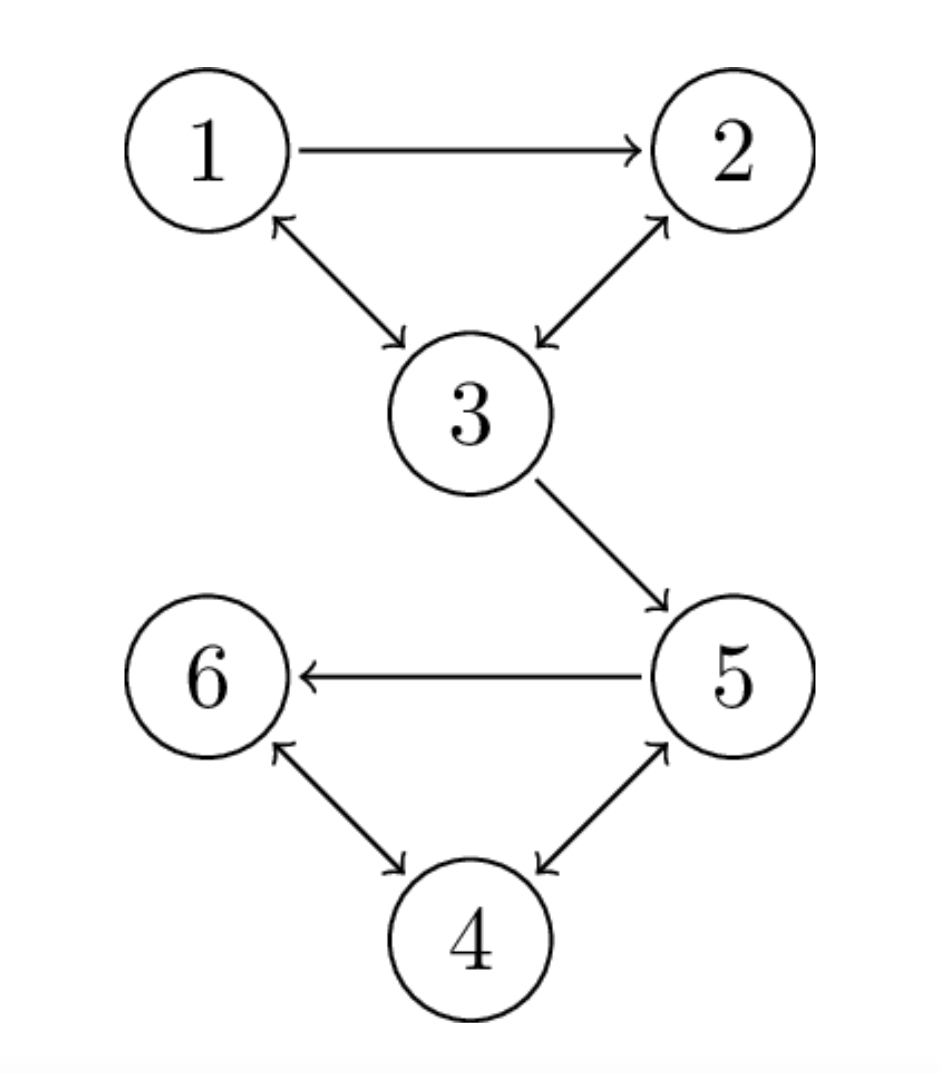
\includegraphics[width=0.20\textwidth]{graph1.png}
    \caption{Stocastic Matrix Graph}
    \label{fig:graph1}
\end{figure}

\noindent To start, we defined a 6-node directed graph where each page links to one or 
more pages, as shown in Figure ~\ref{fig:graph1}. From this, we constructed
the hyperlink matrix $\boldsymbol{H}$, where each non-zero entry $\boldsymbol{H}_{ij}$
is equal to $\frac{1}{|P_{ij}}$, the reciprocal of the number of outbound links
from page $P_j$. This matrix represents the probability that an agent on
page $j$ clicks through to page $i$:
\begin{equation}
    \boldsymbol{H}=\begin{pmatrix}
        0&0&1/3&0&0&0\\
        1/2&0&1/3&0&0&0\\
        1/2&1&0&0&0&0\\
        0&0&0&0&1/2&1\\
        0&0&1/3&1/2&0&0\\
        0&0&0&1/2&1/2&0
    \end{pmatrix}
\end{equation}

\noindent We initialized the PageRank vector $\boldsymbol{x}_0$ with equal
values and assumed that each page is equally likely to be visited at first:
\begin{equation}
    \boldsymbol{x}_0=
        \begin{pmatrix}
            1/6\\1/6\\1/6\\1/6\\1/6\\1/6
        \end{pmatrix}
\end{equation}
\noindent We then applied the iterative update rule $\boldsymbol{x}_{n+1}=\boldsymbol{H}\boldsymbol{x}_n$
until the rank vector converged below a given tolerance to simulate an agent moving
moving through the web graph via the links. We visualized the convergence of the PageRank vector by 
plotting each page's rank score for each iteration, which allowed us to track how the scores
changed until they reached a steady state. Our results are shown in Figure~\ref{fig:conv1}.
\begin{figure}[H]
    \centering
    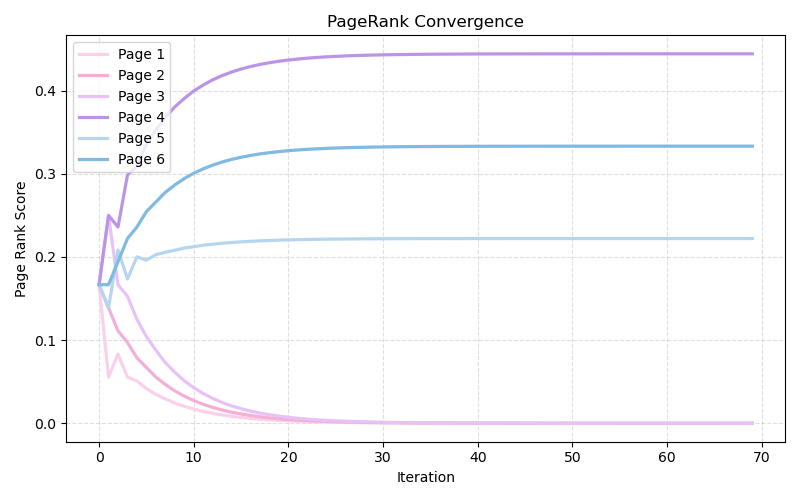
\includegraphics[width=0.4\textwidth]{convergence1.png}
    \caption{PageRank convergence for graph 1.}
    \label{fig:conv1}
\end{figure}
\noindent The convergence of the iterative method is a direct consequence of the 
underlying theory of stochastic matrices. According to Theorem~4.9, if 
$\boldsymbol{H}$ is an $n\times n$ stochastic matrix and $\boldsymbol{x}_0$ is 
some initial vector, then the system defined by the difference equation 
$\boldsymbol{x}_{n+1}=\boldsymbol{H}\boldsymbol{x}_n$ converges to a unique 
steady-state vector. This limit corrresponds to the eigenvector $\boldsymbol{v}_1$ 
associated with eigenvalue $\lambda=1$, since all the other eigenvalue 
components vanish as $k\to\infty$:
\begin{equation}
    \boldsymbol{x}_\text{equilibrium}=\lim_{k\to\infty}\boldsymbol{H}^k\boldsymbol{x}_0=c_1\boldsymbol{v}_1
\end{equation}
\noindent Theorem~4.9 greatly simplifies the PageRank iterative process.
Instead of repeatedly applying $\boldsymbol{x}_{n+1}=\boldsymbol{H}\boldsymbol{x}_n$,
we can directly compute the dominant eigenvector of $\boldsymbol{H}$ corresponding
to the eigenvalue $\lambda=1$. This vector represents the steady-state solution
and results in the same PageRank distribution as the limit of the iterative method. 

Both the iterative difference equation and the eigenvector method yield the
same steady-state PageRank vector:
\begin{equation}
    \boldsymbol{x}_\text{converged}=
    \begin{pmatrix}
        0\\0\\0\\4/9\\2/9\\1/3
    \end{pmatrix}
\end{equation}

\noindent We applied the PageRank algorithm to a second web graph consisting of
eight interconnected pages, as shown in Figure~\ref{fig:graph2}. 


\begin{figure}[H]
    \centering
    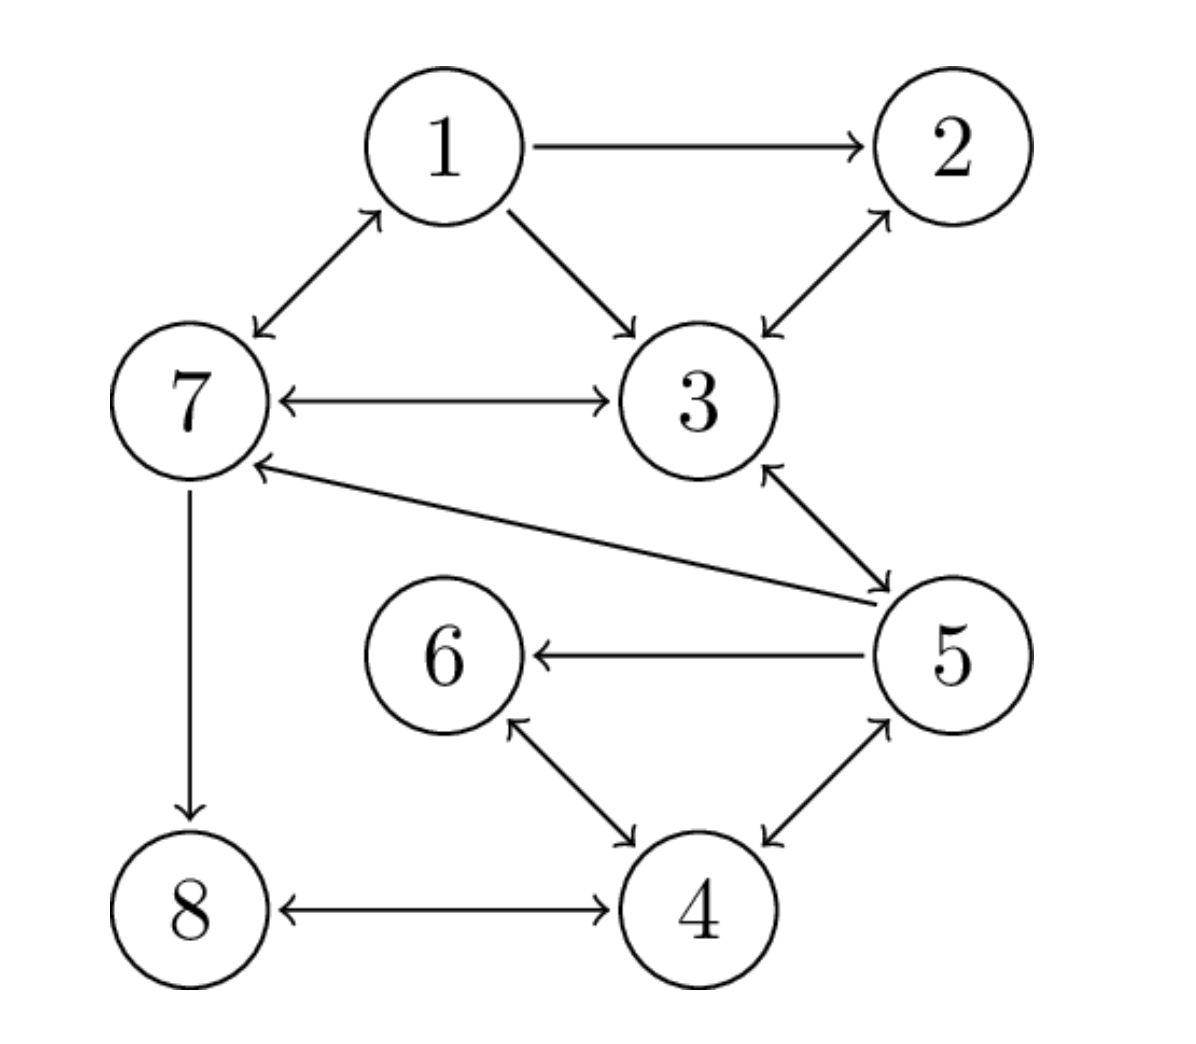
\includegraphics[width=0.25\textwidth]{graph2.png}
    \caption{example graph 2.}
    \label{fig:graph2}
\end{figure}

 The 
corresponding hyperlink matrix $\boldsymbol{H}$ and initial uniform state
vector $\boldsymbol{H}$ are defined below.


\begin{equation}
    \boldsymbol{H}=\begin{pmatrix}
        0 & 0 & 0 & 0 & 0 & 0 & 1/3 & 0 \\
        1/3 & 0 & 1/3 & 0 & 0 & 0 & 0 & 0 \\
        1/3 & 1 & 0 & 0 & 1/4 & 0 & 1/3 & 0 \\
        0 & 0 & 0 & 0 & 1/4 & 1 & 0 & 1 \\
        0 & 0 & 1/3 & 1/3 & 0 & 0 & 0 & 0 \\
        0 & 0 & 0 & 1/3 & 1/4 & 0 & 0 & 0 \\
        1/3 & 0 & 1/3 & 0 & 1/4 & 0 & 0 & 0 \\
        0 & 0 & 0 & 1/3 & 0 & 0 & 1/3 & 0 \\
    \end{pmatrix}
\end{equation}

\begin{equation}
    \boldsymbol{x}_0=\begin{pmatrix}1/8\\1/8\\1/8\\1/8\\1/8\\1/8\\1/8\\1/8\end{pmatrix}
\end{equation}

\noindent Using both the iterative update method and the dominant eigenvector
approach, we computed the steady-state PageRank distribution. The convergence
behavior of the iterative method is shown in Figure~\ref{fig:conv2}

\begin{figure}[H]
    \centering
    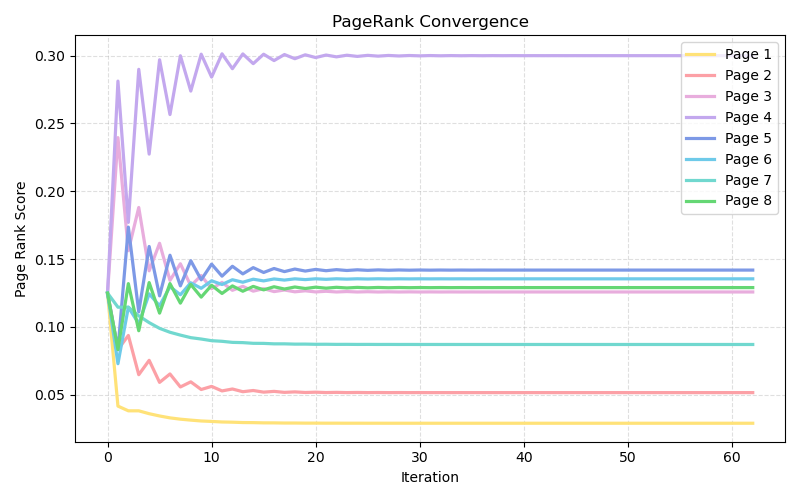
\includegraphics[width=0.4\textwidth]{convergence2.png}
    \caption{PageRank Convergence for graph 2.}
    \label{fig:conv2}
\end{figure}

\noindent Using both the iterative difference equation and the dominant eigenvector
method, we arrive at the same steady-state PageRank vector:

\begin{equation}
    \boldsymbol{x}_\text{converged}=
    \begin{pmatrix}
        0.0290\\
        0.0516\\
        0.1258\\
        0.3000\\
        0.1419\\
        0.1355\\
        0.0871\\
        0.1290
    \end{pmatrix}
\end{equation}
\section{Results} \label{sec:results}

\noindent This distribution for the first web graph reflects the long-term behavior of an agent nagivating the web graph. Based on the values, we rank the pages in order of
importance as follows:
$$
\text{Page 4} > \text{Page 6} > \text{Page 5} > \text{Page 1} = \text{Page 2} = \text{Page 3}
$$
\noindent 

We know that after a long enough time span, $\frac{4}{9}$ of a group of people will end up in Page 4, $\frac{2}{9}$ of a group of people will end up in page 5, and $\frac{1}{3}$ of a group prople will end up in Page 1. No one will end up on Page 1, 2, and 3. 

\noindent From this second web graph result, we rank the pages in order of importance:
$$
\text{Page 4} > \text{Page 5} > \text{Page 6} > \text{Page 8} > \text{Page 3}
$$
$$
> \text{Page 7} > \text{Page 2} > \text{Page 1}
$$
\noindent Page~4 is the most dominant, whereas Page~1 has the lowest influence
in the network. In order word most people will end up on page 4 and the least amount of people will end up on page 1 given a long enough timespan. 

\section{Summary and Conclusion} \label{sec:summary}


\noindent To summarize, we implemented two numerical approaches to compute the
PageRank vector. The first was an iterative method that started from a uniform
initial distribution $\boldsymbol{x}_0$ and repeatedly applied the
update equation $\boldsymbol{x}_{n+1}=\boldsymbol{H}\boldsymbol{x}_n$ until the
difference between successive iterations fell below a convergence threshold.
The second approach used Theorem~4.9, which states that the steady-state 
distribution is the dominant eigenvector of the stochastic matrix $\boldsymbol{H}$.
Both methods gave identical results, which confirms the accuracy of our
implementation to describe long term internet behavior. We performed all computations in Python using \texttt{NumPy}
and visualized convergence behavior with \texttt{matplotlib}.

The biggest limitation is that each iteration is assumed to be indepedent, which means that the current page and previous that the user is on does not influence the next page the user will explore. This condition might of held when the internet was more decentralized. Given the rise of modern recommendation algorithm on platforms that tries to maximize user retention, this assumption doesn't hold true.

Another limitation is that the PageRank matrix \textbf{H} must be ergodic, such as the one that we've shown in the article. In order to solve this issue a pertubation can be made to the original matrix be made to make all matrixes ergodic. This is done by introducing a dampening factor $\alpha$ which represent the dampening factor, J is a ones matrix, and n is the number of pages. 

\begin{equation}
  \label{eq:} \hat{H} = (1 - \alpha) H + \frac{\alpha}{n} J
\end{equation}

This pertubation represents the chance that the user has of jumping to another page randomly. It has a nice property of preventing loops from forming, while also summing the probabilities for one page to jump to another page up to one which defines a stocastic matrix.

\subsection{Acknowledgements}
We thank Professor Mitra for his guidance and instruction throughout the course,
as well as the teaching assistants for their helpful feedback. We also
acknowledge the Department of Physics for providing an excellent academic foundation 
to support this work. This work was completed as part of the requirements for 
C S 323E: Elements of Scientific Computing at the University of Texas at Austin.

\newpage
\bibliographystyle{aasjournal}
\bibliography{refs}

\end{document}
